% !TeX spellcheck = en_US
% !TeX encoding = UTF-8
\documentclass{ifacconf}

% ------------------- debug cleveref and ifacconf -----------------------------
\newcounter{part}
\counterwithin*{section}{part}
%% ===================== packages ============================================
\usepackage[utf8]{inputenc}
\usepackage{amsmath,amssymb,dutchcal,mathtools,siunitx,physics,etoolbox}
\usepackage{booktabs,graphicx,xcolor,colortbl,natbib,tikz,epstopdf}
\usepackage[capitalize]{cleveref}
\usepackage[qtmarkupright]{glosmathtools}
%% =============== preamble ==================================================
%% ---------------- tikz -----------------------------------------------------
\usetikzlibrary{arrows,shapes.geometric}
%%generate seperate PDF for each tikz (compile with pdflatex -shell-escape) :
%\usetikzlibrary{external}
%\tikzexternalize[prefix=fig/]
%% ------------- glosmathtools -----------------------------------------------
\newignoredglossary{ignoredglos} % vectors are not printed in nomenclature
\loadglsentries{mpcPackageJulia_glos}
%% ----------------- amsmath -------------------------------------------------
\DeclareMathOperator{\diag}{diag}
%% ============================================================================

\begin{document}
\begin{frontmatter}

\title{ModelPredictiveControl.jl: toward democratizing advanced process control solutions}

\author[First]{Francis Gagnon} 
\author[First]{Alex Thivierge} 
%\author[Second]{André Desbiens}

\address[First]{Process Observation and Optimization Laboratory (LOOP), Université Laval, Quebec City, G1V 0A6, Canada}
\address[Second]{Process Monitoring Automation and Control group (PMAC), Pfizer Canada ULC, Montreal, H9J 2M5, Canada}

\begin{abstract} 
Sit commodo ipsum nulla eu excepteur sit ut minim voluptate et eu velit sint. Lorem et amet incididunt officia id. Nulla magna fugiat incididunt veniam sunt excepteur in esse nulla et aliquip non magna deserunt. 
\end{abstract}

\begin{keyword}
Model-based Control
\end{keyword}

\end{frontmatter}

% !TeX encoding = UTF-8
% !TeX spellcheck = en_US
\section{Introduction}

The process control community, both in the academic and industrial sectors, has largely relied on MATLAB toolboxes and commercial solutions for designing, simulating and implementing closed-loop systems \citep{optimMatlab}. The ecosystem developed by MathWorks\texttrademark\ is rich, mature, cohesive, and well documented, but their licensing policy can be unaffordable for smaller organizations. Moreover, because it is a proprietary software, the source code of many functions is not available. This is an issue for scientific research, where reproducibility and transparency is a key aspect. The dependency on a single vendor also raises concerns about the long-term support of third-party control software products. Lastly, like any interpreted languages e.g., Python, its performance can be suboptimal for computationally intensive tasks, especially for time-critical applications like real time optimization and model predictive control \citep{matlabPythonJulia, juliaML}. Code generation mitigates this issue, but it creates other problems like additional licensing fees, the difficulty to debug the generated code, and the restriction to a subset of the language.

Julia is relatively new programming language specialized for scientific and numerical computing. The just-ahead-of-time compiler can reach performance comparable to C and Fortran, while exhibiting a modern and expressive syntax like MATLAB and Python \citep{juliaPaper}. The built-in read-eval-print-loop (REPL) allows to interactively test code and inspect variables, mimicking the development workflow of an interpreted language. It also includes a package manager with a general registry, which makes it easy to share, install or update code. Moreover, the environment is free and open-source and it can be used for commercial purposes without any licensing fees. The ecosystem is still young, but a control toolbox (\texttt{ControlSystems.jl}), a system identification (\texttt{ControlSystemIdentification.jl}) and an optimization (\texttt{JuMP.jl}) packages are already available \citep{controlsystems, jump}. There is no free and open-source model predictive control (MPC) toolset available yet in the official registry of Julia, which is the gap this work fills.

This paper presents an MPC package for Julia. It aims to provide a simple, clear and modular framework to quickly design and test predictive controllers in Julia, while preserving the flexibility for advanced real-time optimization. For now, the package does particularly endeavor for original methodological scientific contributions or bleeding edge technologies like collocation methods or robust MPC, but rather to improve the accessibility to advanced process control, both for the academic and industrial community. With the exception of the petrochemical sector, many facilities still run their processes entirely in open-loop or with simple local controllers \citep{gapMPC}. Advanced process control can significantly reduce the waste in raw material and energy consumption. This is highly needed in the context of climate changes and the increasing scarcity of resources.

It focuses on modern MPCs that rely on a closed-loop state estimator for the feedback. The package currently implements the Luenberger observer and all the classical Kalman-type filters. It also incorporates an internal model control structure, as a more traditional approach. In addition, the analog of predictive control but for state estimation, the moving horizon estimator (MHE), is also available to solve constrained estimation problems. The user can also provide its own feedback strategy by defining a new state estimator subtype.

Linear plant models are automatically augmented with an adequate representation of the unmeasured disturbances based on observability (customizable). For the nonlinear case, the user chooses to add integrated white noise on the input or output for each channel. The \texttt{JuMP.jl} interface allows changing the solver quickly among  many open-source and commercial optimization software (local and global). As generic Julia functions can be differentiated using automatic differentiation , the gradient and Jacobian of the objective/constraint function for nonlinear MPCs are computed automatically with the machine precision. This also applies for the extended Kalman Filter. 

Additionally, by leveraging the multiple dispatch paradigm of Julia, nonlinear controllers based on linear models (e.g., economic MPC) evaluate the predictions with matrix algebra instead of a \texttt{for} loop, which is generally more efficient especially for the constraint handling. More precisely, the package functions dispatch on both the types of the controller and the plant model to select the most efficient implementation. Both soft and hard constraints on inputs, input increments, outputs, and terminal states are supported. The MHE state and noise estimates also support constraint relaxation.

The next section presents the structure and the main features of the package. The following one present two case studies to illustrate the syntax and benchmark the performances: a linear and a nonlinear controller design.
% !TeX encoding = UTF-8
% !TeX spellcheck = en_US

\section{Materials and Methods}
\label{sec.mat_method_simple}

Aliqua aliquip ipsum aute qui ad culpa voluptate in ea. Ipsum aliquip cillum do anim in. Enim eiusmod ipsum elit velit irure laborum ipsum veniam non sint.

Tempor enim anim ut velit cillum veniam velit non quis mollit do occaecat. Est consectetur enim ipsum qui sunt qui aute veniam veniam occaecat reprehenderit officia. Sint non pariatur esse ex adipisicing cillum veniam. Labore qui enim nostrud aute est enim qui irure dolore. Cupidatat enim occaecat labore aliquip sunt exercitation.

Deserunt minim irure in est laboris pariatur esse irure elit aliquip Lorem velit amet nostrud. Excepteur exercitation dolor dolore proident elit cillum. Commodo quis Lorem eu cupidatat veniam ea eu. Excepteur esse pariatur aliquip officia occaecat pariatur irure amet est elit occaecat proident ut.

Amet culpa dolor dolor irure duis consequat amet. Voluptate nulla pariatur ipsum voluptate. Minim do tempor aute veniam occaecat non enim voluptate veniam aliqua duis proident. Ex cillum aliqua consectetur labore incididunt mollit amet sunt commodo. Eiusmod aliquip aliquip sunt ut minim veniam Lorem aliquip enim culpa dolore dolor enim dolore.

Laboris cupidatat deserunt mollit ullamco. Anim dolore pariatur cillum esse. Ea mollit deserunt cillum deserunt velit commodo sit cupidatat. Commodo adipisicing occaecat Lorem cupidatat et. Exercitation esse quis ex irure laboris.

Et quis fugiat reprehenderit aute cillum esse laboris nostrud. Proident sunt quis nulla labore consectetur do pariatur nisi id aute. Enim consequat aliqua mollit eiusmod commodo sit quis ut veniam. Et ea aute magna aliquip ipsum. Dolore incididunt deserunt nisi incididunt ea in aliquip consectetur laborum. Ipsum voluptate excepteur exercitation eu esse sit consectetur commodo amet.

Adipisicing minim tempor reprehenderit laboris sit ex tempor exercitation qui. Aliquip elit occaecat enim anim veniam excepteur occaecat anim Lorem quis ex. Non sit ea sunt occaecat minim. Nisi elit laborum et esse ex sint aute velit dolor. Enim qui velit Lorem occaecat ad consectetur dolore qui ut id laborum eiusmod.

Veniam amet ea aliquip proident amet mollit ad incididunt aliqua proident. Cupidatat do sint sunt do tempor in consectetur pariatur laborum commodo. Laboris qui excepteur exercitation nisi deserunt nisi tempor labore cillum non adipisicing duis adipisicing. Laborum eu adipisicing adipisicing reprehenderit ipsum elit ipsum fugiat proident.
% !TeX encoding = UTF-8
% !TeX spellcheck = en_US
\section{Results and Discussion}
\label{sec.results_simple}

Laboris exercitation sunt adipisicing laboris nulla ad occaecat irure magna voluptate. Veniam eu labore Lorem anim nostrud minim Lorem fugiat nulla. Non anim veniam laborum deserunt adipisicing cillum aliquip deserunt pariatur consectetur consequat irure. Dolor aute incididunt quis magna. Dolor nostrud exercitation duis sunt nulla adipisicing enim laborum ex ut esse ad. Incididunt exercitation velit ea elit ut laboris eu amet.

Minim magna culpa ipsum do proident cillum sit. Officia ad et consequat do magna nostrud irure nostrud. Ipsum sunt adipisicing Lorem sunt tempor ex veniam consequat veniam ipsum. Aliquip voluptate labore mollit duis id mollit nulla id ipsum. Velit esse nisi qui pariatur ad nostrud.

Aute minim anim culpa minim aliquip sint laboris sunt. Ea ex tempor irure officia laborum est aliquip nostrud quis do. Lorem cupidatat mollit do officia aute in est cillum cillum consectetur laborum pariatur. Id tempor minim eiusmod ex laboris. Aute aliquip cupidatat nostrud aute dolor mollit ex commodo do excepteur dolor irure. Ut veniam amet id excepteur excepteur velit laboris aliqua sit occaecat irure dolor labore.

Proident ad minim magna minim excepteur reprehenderit elit id ipsum amet velit sunt aute aute. Consectetur excepteur velit quis aliqua sint laborum veniam minim proident. Veniam proident laboris aute deserunt do do amet qui pariatur occaecat cillum. Minim magna in et laborum ipsum deserunt pariatur cupidatat ipsum veniam aliqua elit. Aliqua id proident fugiat nisi esse eu nulla sint qui reprehenderit aliqua sunt. Cillum duis anim sit velit dolore.

\begin{table}[tb]
	\caption{Simplified model parameters for batch fluidized bed drying}
	\label{tab.simple_params}
	\centering
	% !TeX spellcheck = en_US

\begin{tabular}{l l l l}
	
\toprule %=======================================================================

parameter 			& value 	   		& \shortstack[l]{standard\\deviation} & units  \\

\midrule %-----------------------------------------------------------------
					
\glsub{chi}{0}    	& \num{0.15e-2}		& -- 					& --		\\

%--------------------------------------------------------------------------

\rowcolor{blue!10}
\gls{a1}			& \num{9.26e-5}		& \num{0.04e-5}		%
										& \si{\per\meter\cubed} \\
\rowcolor{blue!10}
\gls{b1}			& \num{4.54e-2}		& \num{0.05e-2}		%
										& \si{\degreeCelsius\per\meter\cubed} \\
\rowcolor{blue!10}					
\gls{b2}			& \num{2.56e-05}	& \num{0.02e-05}	%
										& \si{\per\meter\cubed}	 \\

%--------------------------------------------------------------------------

\rowcolor{blue!10}
\gls{nu}			& \num{3.48}		&  \num{0.12}		& -- \\		
\rowcolor{blue!10}
\glsub{chi}{pc}		& \num{2.33e-2}	 	&  \num{0.06e-2}	& -- \\
				
%-------------------------------------------------------------------------

\gls{alpha}   	   	& \num{4.90e-3} 	& --			& --  \\
\gls{beta}			& \num{5.70e-2}		& -- 			& \si{\per\degreeCelsius}\\

%----------------------------------------------------------------------------

\gls{tau}			& \num{86.7}		&--				& \si{\second}  \\

\bottomrule %====================================================================
	
\end{tabular}

\end{table}

Occaecat Lorem commodo in minim consectetur voluptate nostrud enim tempor incididunt laborum occaecat. Aliqua non et nulla voluptate amet sunt. Laboris nisi consequat cupidatat est consequat deserunt ipsum.

Fugiat eu id qui nostrud adipisicing aute quis qui labore. Officia pariatur sunt ex deserunt culpa. Cupidatat est Lorem laborum laboris do culpa labore aliqua.

\begin{figure}[tb]
	\centering
	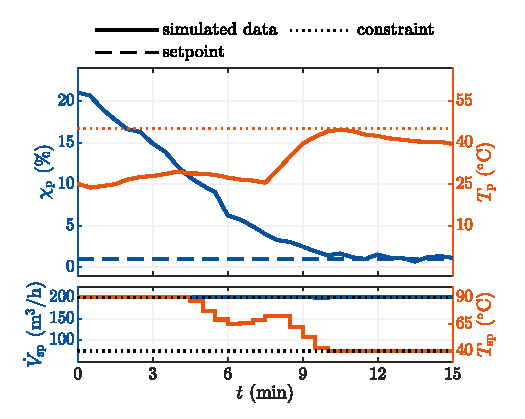
\includegraphics{fig/batchFBD_simpleNMPC.eps}
	\caption{Simplified predictive control results on simulator}
	\label{fig.batchFBD_simpleNMPC}
\end{figure}


\cref{fig.batchFBD_simpleNMPC} Ea cillum commodo labore eiusmod non ut eu labore nulla Lorem sint. Labore proident ut enim exercitation officia voluptate laborum fugiat quis ex duis consectetur occaecat consectetur. Velit minim sint est id occaecat aute incididunt consequat. Eu minim veniam tempor eu ullamco duis et Lorem commodo in dolore occaecat. Et proident quis qui qui qui reprehenderit laborum consequat fugiat nisi dolore veniam excepteur velit.

Sunt eu tempor veniam ullamco sit nulla enim ea. Anim mollit sint non dolore. Cillum mollit deserunt sint adipisicing cillum in. Fugiat mollit cupidatat Lorem nisi et ex ipsum dolor laborum adipisicing cillum culpa velit incididunt. Excepteur culpa quis mollit irure laboris ad tempor id sint tempor. Anim officia qui nulla ad eiusmod incididunt veniam amet dolore do reprehenderit. Reprehenderit culpa esse dolore magna nostrud tempor.

Voluptate velit magna sit nulla laboris. Aute ut sit veniam ut. Anim est exercitation dolore id deserunt officia qui nulla sit ea veniam enim ut.

Voluptate voluptate occaecat incididunt deserunt. Nisi aliquip officia laborum consequat tempor. Nostrud nisi cupidatat Lorem minim ullamco excepteur commodo aliqua sint laborum veniam esse qui dolor. Sint consequat ullamco quis proident in nulla quis do. Cillum dolore deserunt aliqua tempor id laboris sunt dolor consequat fugiat eu veniam nostrud pariatur. Nulla cupidatat excepteur exercitation mollit ex commodo est in quis cillum incididunt aliquip esse cillum. Adipisicing do Lorem labore officia nulla id.
% !TeX encoding = UTF-8
% !TeX spellcheck = en_US
\section{Conclusion}

This paper introduced the \texttt{ModelPredictiveControl.jl} package, a free and open-source package for advanced process control in Julia. It relies on \texttt{ControlSystems.jl} and \texttt{JuMP.jl}, two powerful frameworks for computer-aided control system design and mathematical optimization, respectively. The new state estimator and predictive controller types are designed to be easy to use, clear and modular. The main features of the package were described and illustrated with two case studies. A benchmark comparison with the equivalent MATLAB toolbox exposes its computational efficiency, without any code generation, and thus avoiding the two-language problem. The package is still under active development and contributions are welcome. Short-term developments will focus on implementing estimators in the current form to eliminate the one-sample time delay when possible. Recent developments on abstraction interfaces to automatic differentiation libraries could be also integrated to facilitate the testing of other approaches like reverse- or mixed-mode.

\begin{ack}
Culpa in deserunt proident tempor non. Duis et esse pariatur esse qui duis exercitation ullamco aliquip. Dolore ipsum sint consequat enim laborum duis anim cupidatat.
\end{ack}

\bibliography{mpcPackageJulia_bibfile}


\end{document}